% pilot
The Rhode Island Board of Elections performed a pilot audit in Providence 
in February 2022. The contest audited was a single yes-or-no question in the November 202 1 election: Portsmouth's
Issue 1, "School Construction and Renovation Projects". The question had announced margin $25.67\%$ and the audit used risk-limit $10\%$.

A first round size of $140$ ballots with large probability of stopping ($95\%$) was selected
in order to give the potential for more interesting analysis afterwards; the large margin 
made a first round with large stopping probability practical.
Selection order was tracked for the sake of analysis.
As expected, the audit concluded in the first round with a \Providence risk of $4.18\%$. Table~\ref{tab:pilot-risks} shows risk measures for the drawn sample using \Minerva and \BRAVO (both EoR and SO).

\begin{table}
\begin{center}
\begin{tabular}{ |c|c|c|c|c| } 
\hline
%\diagbox[dir=NW]{First \\Round \\Size}{RLA}
ballots& \rotatebox{45}{\Providence} & \rotatebox{45}{\Minerva} & \rotatebox{45}{SO \BRAVO} & \rotatebox{45}{EoR \BRAVO} \\
\hline
140 & \bf{4.18\%} & \bf{4.18\%} & \bf{5.41\%} & 36.6\% \\
\hline
\end{tabular}
\end{center}
\caption{Risk measures for the drawn first round of $140$ ballots in the Providence, RI pilot audit. Risks in bold meet the risk-limit ($10\%$) and thus correspond to audits that would stop.}
\label{tab:pilot-risks}
\end{table}

Note that the risk measures shown in Table~\ref{tab:pilot-risk} imply that, for the sample obtained in the pilot audit, an EoR \BRAVO audit would not have been able to stop in the first round, despite the large round size. Further, if the risk limit had been $0.05$ instead of $0.10$, SO \BRAVO also would have required moving on to a second round. 

We can use simulations to better understand typical audit behavior for the margin of this pilot audit and contextualize the results we obtained in the pilot. We run $10^4$ trial audits for several stopping probabilities $p$. Each round size is chosen to give a probability of stopping $p$ assuming the announced tally and given the results of previous rounds. We use the same $10\%$ risk limit and margin of $25.57\%$. 

Figure~\ref{fig:pilot_sims} shows the average number of ballots sampled for each value of $p$ in the simulations. The vertical line denotes the stopping probability of the first round size chosen in the pilot of $140$ ballots. The average number of ballots for such a high stopping probability round schedule is high. blah blah based on plot and some numbers illustrating that point... Of course, average number of ballots is not the only metric that matters when planning an audit. 


\begin{figure}
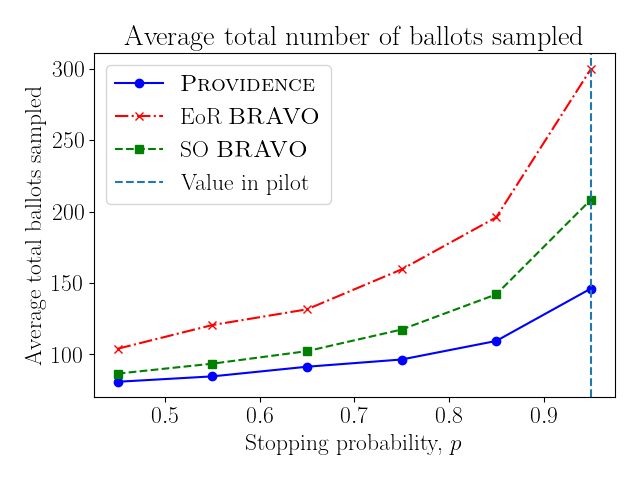
\includegraphics[width=.5\textwidth]{pilot_sims.png}
\caption{The total number of ballots sampled on average in our simulations of audits using the same contest parameters and risk limit as the pilot audit. The average total ballots are shown for various round schedules for which we ran simulations, parameterized by $p$ the conditional stopping probability used to select each round size.}
\label{fig:pilot_sims}
\end{figure}


For this pilot audit, extensive planning of the round schedule was not necessary because the margin was high enough the relatively few ballots were needed even to achieve the high probability of stopping. In Section~\ref{sec:workload} we consider a larger, state-wide contest in Virginia where selecting the round schedule has more significant implications. Virginia also currently uses ballot polling RLAs whereas Rhode Island primarily uses batch comparison RLAs. Some of the ideas introduced in Section~\ref{sec:workload} we do apply to this pilot case as well.

